\begin{figure}
	\centering
	\subfigure[Ground truth trajectory of Bag.0.]{
		\begin{minipage}[t]{0.4\linewidth}
			\centering
			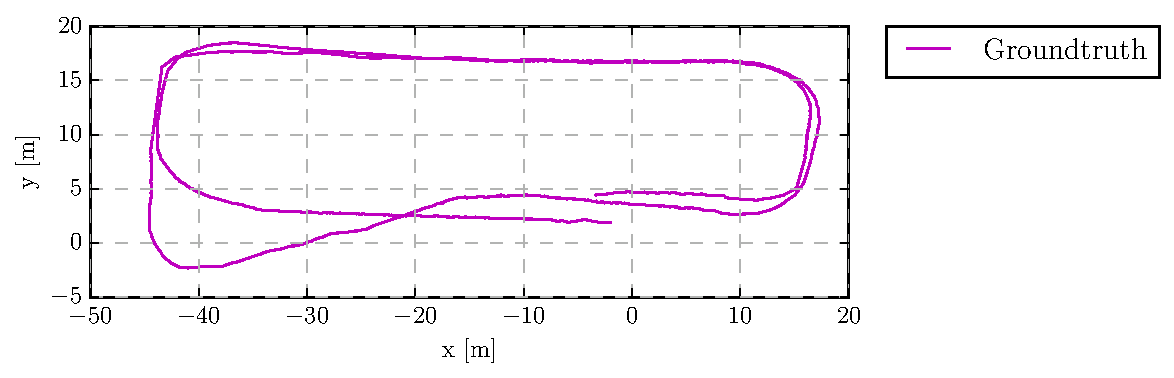
\includegraphics[width=2in]{Chapter4/NTU/0446/plots/trajectory_top_gt_sim3_-1.pdf}
			%\caption{fig1}
		\end{minipage}
	}
	\subfigure[Ground truth trajectory of Bag.1.]{
		\begin{minipage}[t]{0.4\linewidth}
			\centering
			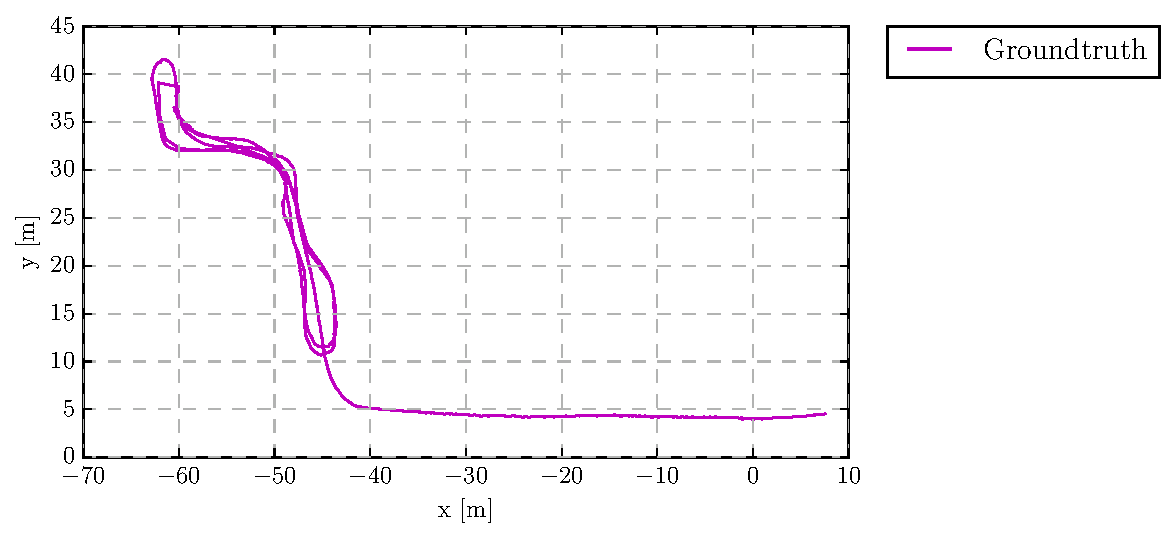
\includegraphics[width=2in]{Chapter4/NTU/0454/plots/trajectory_top_gt_sim3_-1.pdf}
			%\caption{fig2}
		\end{minipage}
	}
	\vfill
	\subfigure[Complete ground truth trajectory of Bag.0 and Bag.1.]{
		\begin{minipage}[t]{\linewidth}
			\centering
			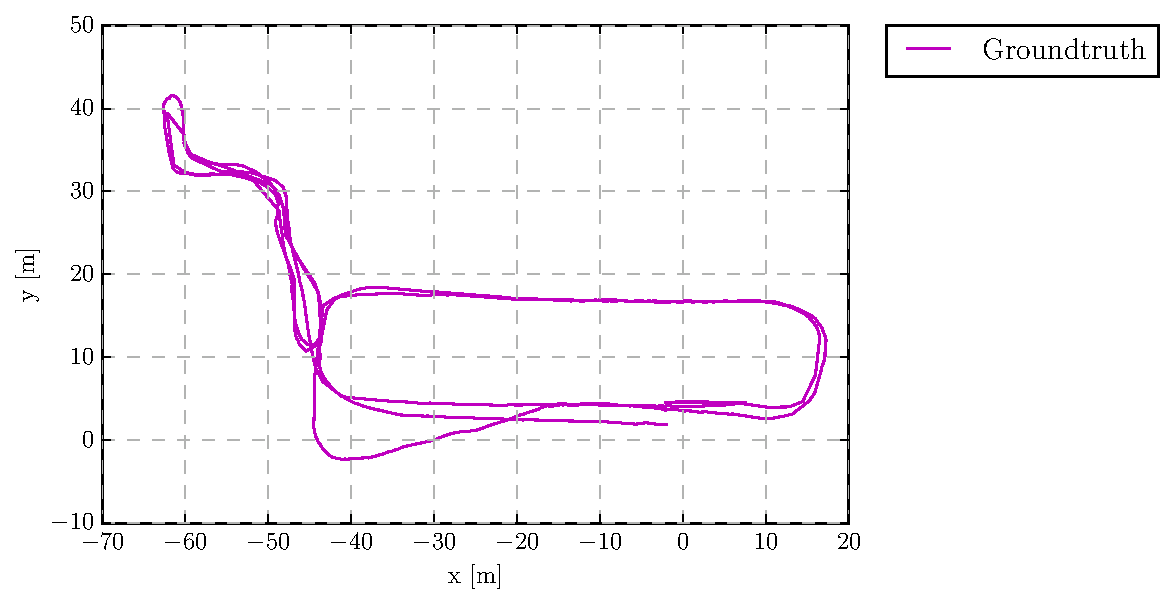
\includegraphics[width=5in]{Chapter4/NTU/server/trajectory_top_gt_sim3_-1.pdf}
			%\caption{fig1}
		\end{minipage}
	}
	\caption{Ground truth trajectory of partial and complete bags of NTU Datasets.}
	\label{fig:ntubag01gt}
\end{figure}

\begin{figure}
	\centering
	\subfigure[Mapping result of Bag.0 compared with ground truth.]{
		\begin{minipage}[t]{0.4\linewidth}
			\centering
			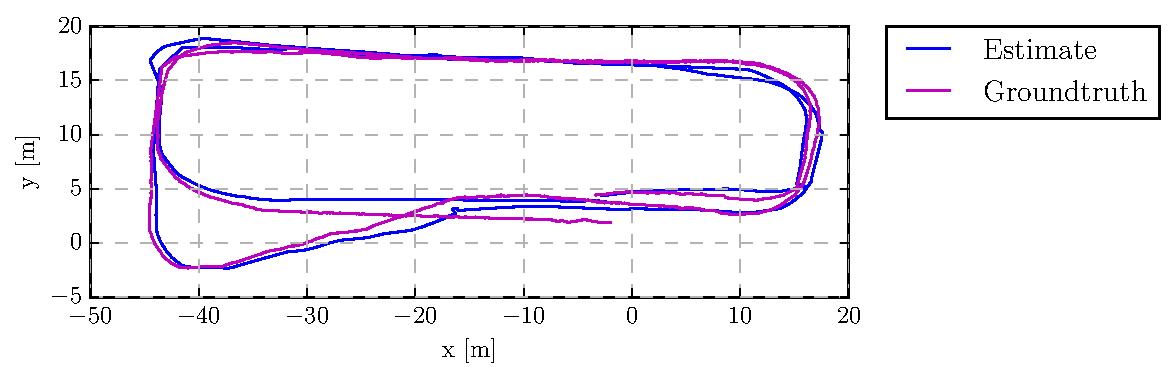
\includegraphics[width=2in]{Chapter4/NTU/0446/plots/trajectory_top_sim3_-1.pdf}
			%\caption{fig1}
		\end{minipage}
	}
	\subfigure[Mapping result of Bag.1 compared with ground truth.]{
		\begin{minipage}[t]{0.4\linewidth}
			\centering
			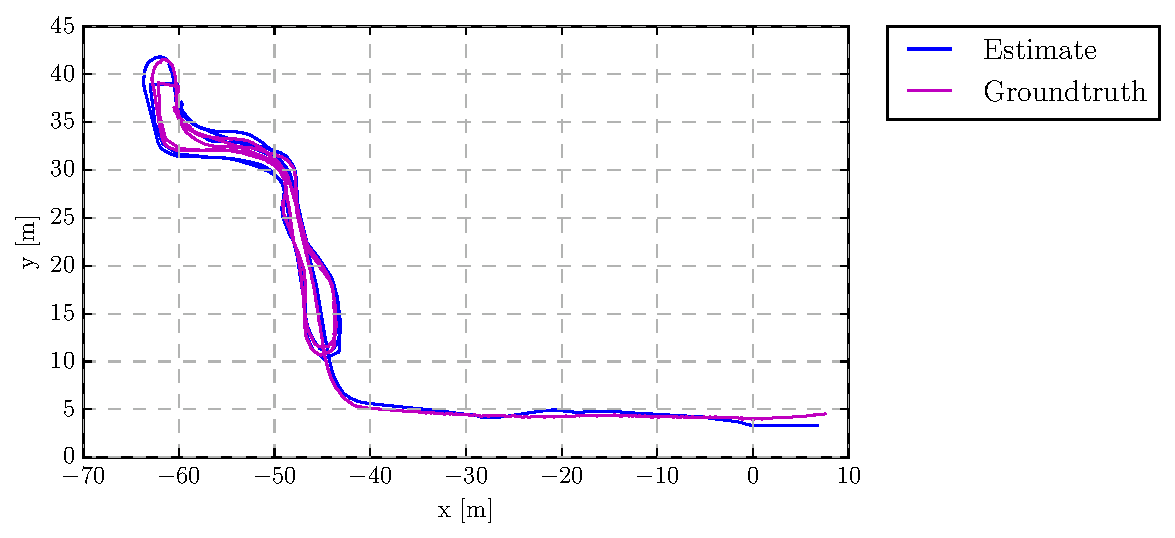
\includegraphics[width=2in]{Chapter4/NTU/0454/plots/trajectory_top_sim3_-1.pdf}
			%\caption{fig2}
		\end{minipage}
	}
	\vfill
	\subfigure[Map Fusion results in server end of Bag.0 and Bag.1.]{
		\begin{minipage}[t]{\linewidth}
			\centering
			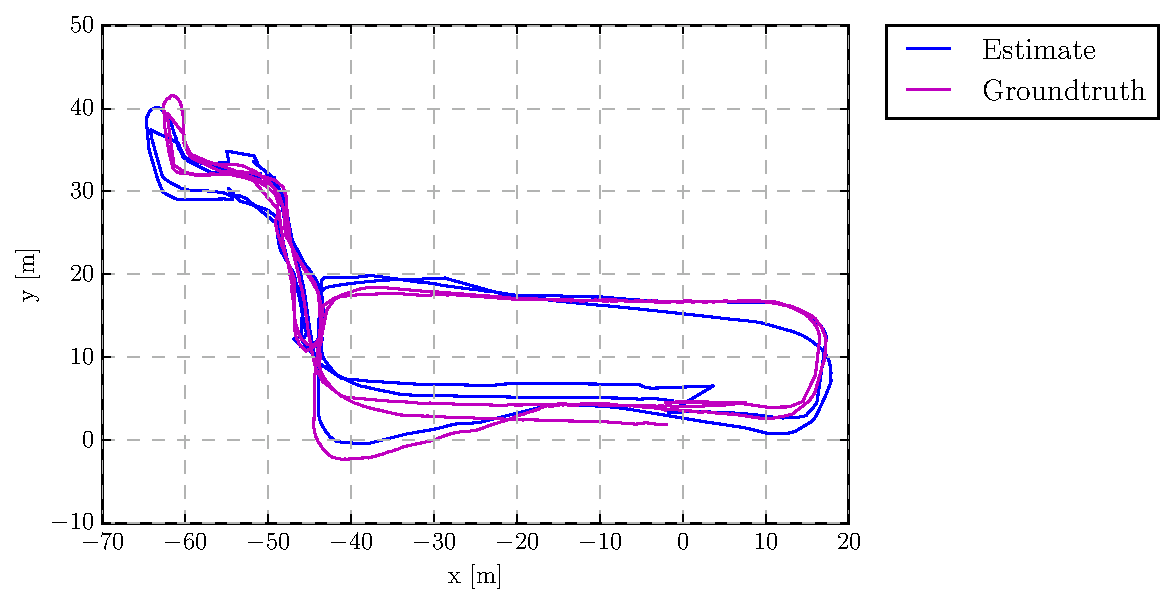
\includegraphics[width=5in]{Chapter4/NTU/server/trajectory_top_sim3_-1.pdf}
			%\caption{fig1}
		\end{minipage}
	}
	\caption{Mapping results of Bag.0 and Bag.1 and the map fusion result of server.}
	\label{fig:ntubag01serverresults}
\end{figure}

\begin{figure}
	\centering
	\subfigure[Relative translation error.]{
		\begin{minipage}[t]{0.4\linewidth}
			\centering
			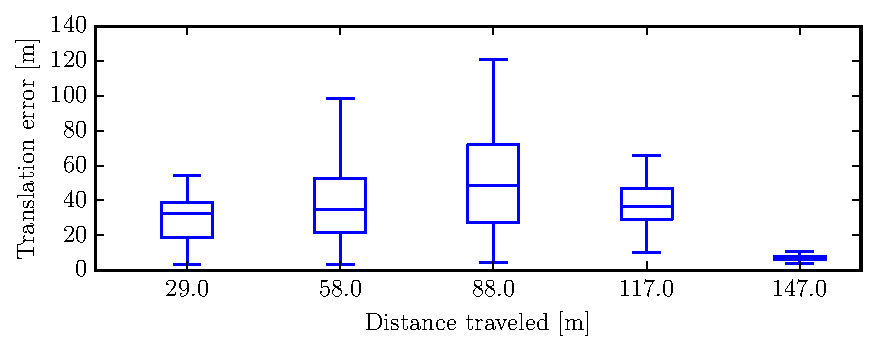
\includegraphics[width=2in]{Chapter4/NTU/0446/plots/rel_translation_error.pdf}
			%\caption{fig1}
		\end{minipage}
	}
	\subfigure[Relative translation error by percent.]{
		\begin{minipage}[t]{0.4\linewidth}
			\centering
			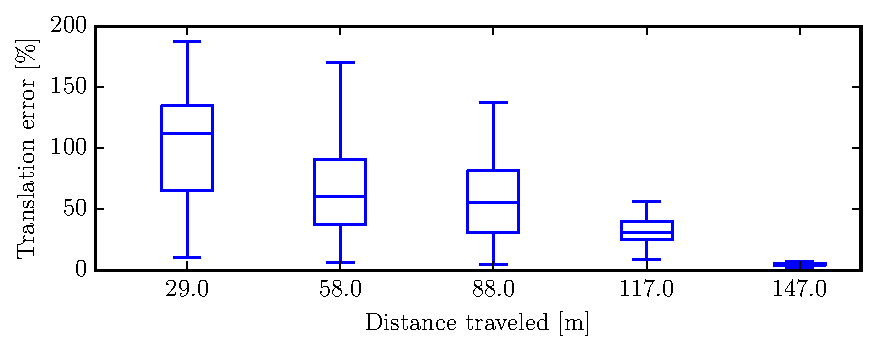
\includegraphics[width=2in]{Chapter4/NTU/0446/plots/rel_translation_error_perc.pdf}
			%\caption{fig2}
		\end{minipage}
	}
	\vfill
	\subfigure[Relative yaw error.]{
		\begin{minipage}[t]{0.4\linewidth}
			\centering
			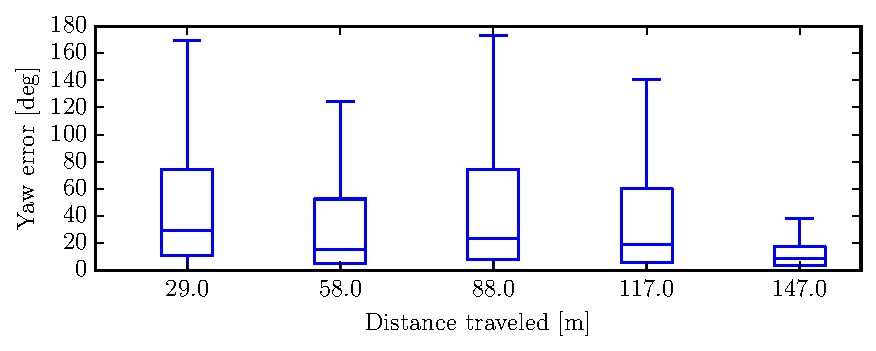
\includegraphics[width=2in]{Chapter4/NTU/0446/plots/rel_yaw_error.pdf}
			%\caption{fig1}
		\end{minipage}
	}
\ifoutputscaleerror
	\subfigure[Scale error.]{
		\begin{minipage}[t]{0.4\linewidth}
			\centering
			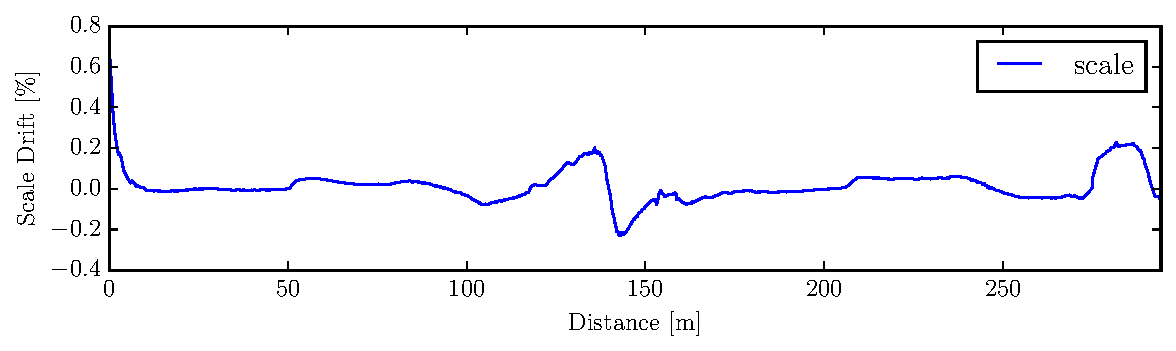
\includegraphics[width=2in]{Chapter4/NTU/0446/plots/scale_error_sim3_-1.pdf}
			%\caption{fig2}
		\end{minipage}
	}
\fi
	\caption{Quantitative evaluation results of mapping Bag.0 of NTU Datasets.}
	\label{fig:ntubag0quanresult}
\end{figure}

\begin{figure}
	\centering
	\subfigure[Relative translation error.]{
		\begin{minipage}[t]{0.4\linewidth}
			\centering
			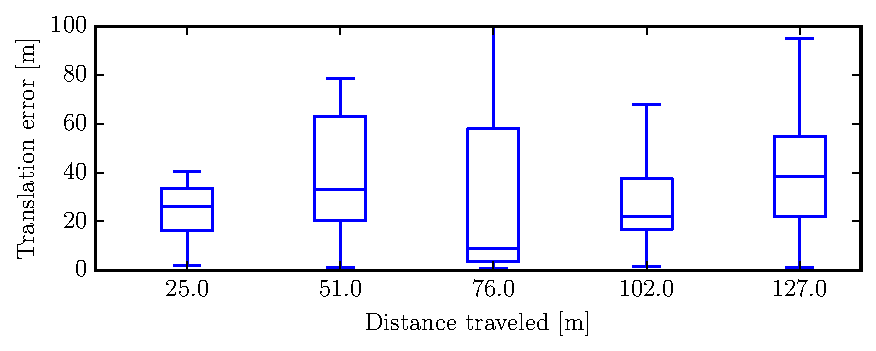
\includegraphics[width=2in]{Chapter4/NTU/0454/plots/rel_translation_error.pdf}
			%\caption{fig1}
		\end{minipage}
	}
	\subfigure[Relative translation error by percent.]{
		\begin{minipage}[t]{0.4\linewidth}
			\centering
			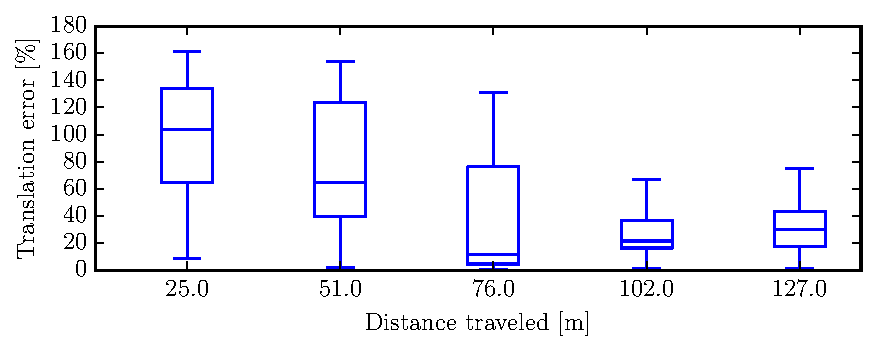
\includegraphics[width=2in]{Chapter4/NTU/0454/plots/rel_translation_error_perc.pdf}
			%\caption{fig2}
		\end{minipage}
	}
	\vfill
	\subfigure[Relative yaw error.]{
		\begin{minipage}[t]{0.4\linewidth}
			\centering
			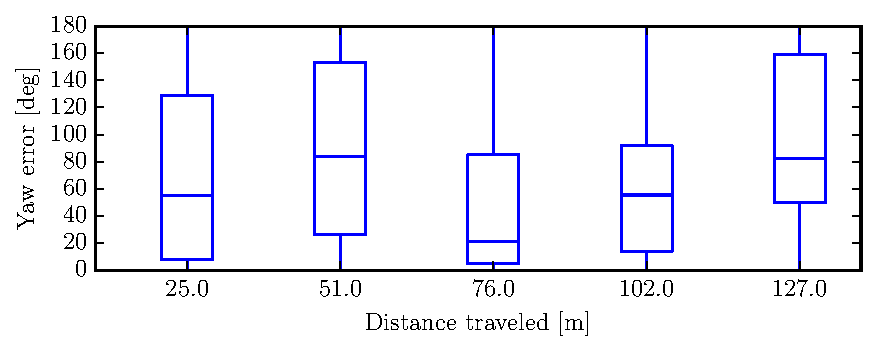
\includegraphics[width=2in]{Chapter4/NTU/0454/plots/rel_yaw_error.pdf}
			%\caption{fig1}
		\end{minipage}
	}
\ifoutputscaleerror
	\subfigure[Scale error.]{
		\begin{minipage}[t]{0.4\linewidth}
			\centering
			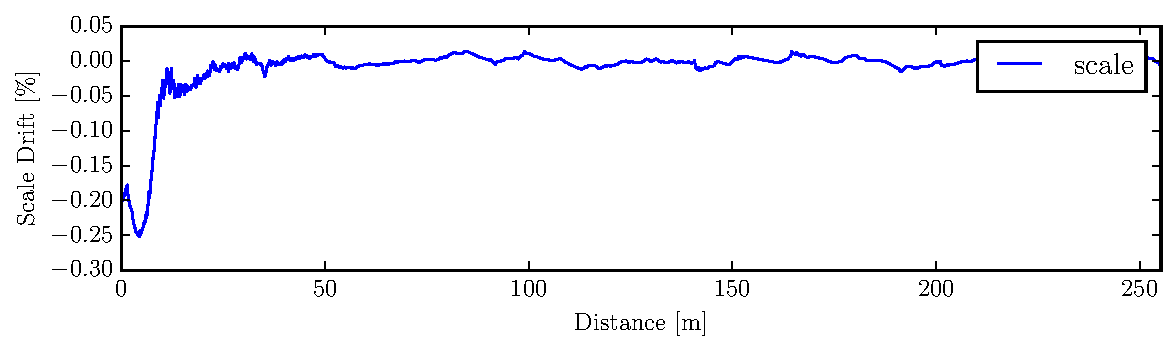
\includegraphics[width=2in]{Chapter4/NTU/0454/plots/scale_error_sim3_-1.pdf}
			%\caption{fig2}
		\end{minipage}
	}
\fi
	\caption{Quantitative evaluation results of mapping Bag.1 of NTU Datasets.}
	\label{fig:ntubag1quanresult}
\end{figure}

\begin{figure}
	\centering
	\subfigure[Relative translation error.]{
		\begin{minipage}[t]{0.4\linewidth}
			\centering
			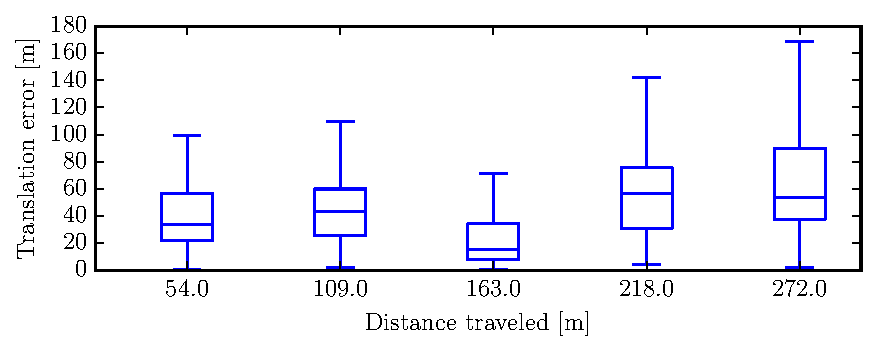
\includegraphics[width=2in]{Chapter4/NTU/server/rel_translation_error.pdf}
			%\caption{fig1}
		\end{minipage}
	}
	\subfigure[Relative translation error by percent.]{
		\begin{minipage}[t]{0.4\linewidth}
			\centering
			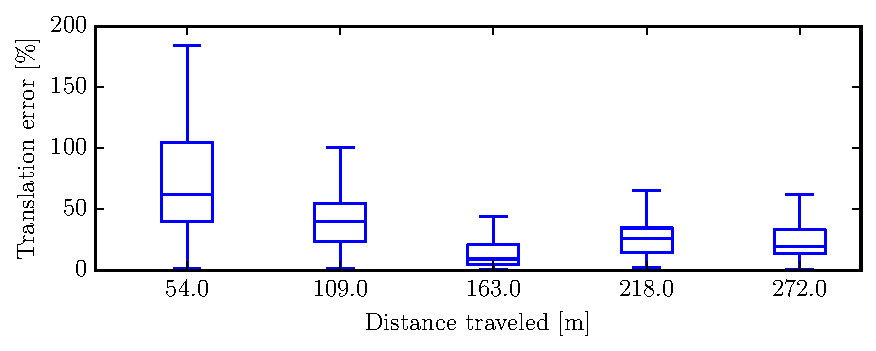
\includegraphics[width=2in]{Chapter4/NTU/server/rel_translation_error_perc.pdf}
			%\caption{fig2}
		\end{minipage}
	}
	\vfill
	\subfigure[Relative yaw error.]{
		\begin{minipage}[t]{0.4\linewidth}
			\centering
			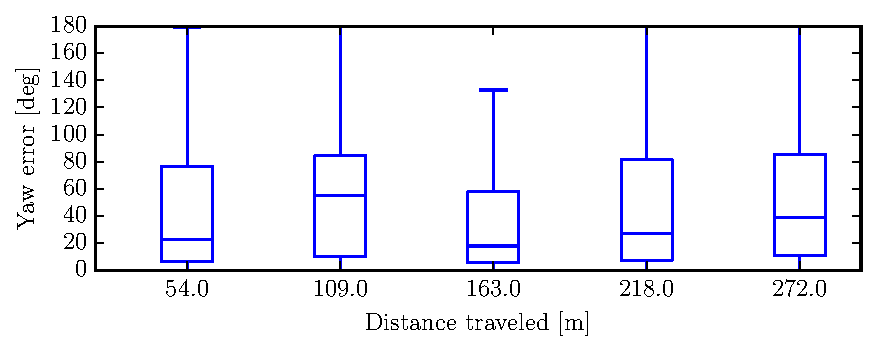
\includegraphics[width=2in]{Chapter4/NTU/server/rel_yaw_error.pdf}
			%\caption{fig1}
		\end{minipage}
	}
\ifoutputscaleerror
	\subfigure[Scale error.]{
		\begin{minipage}[t]{0.4\linewidth}
			\centering
			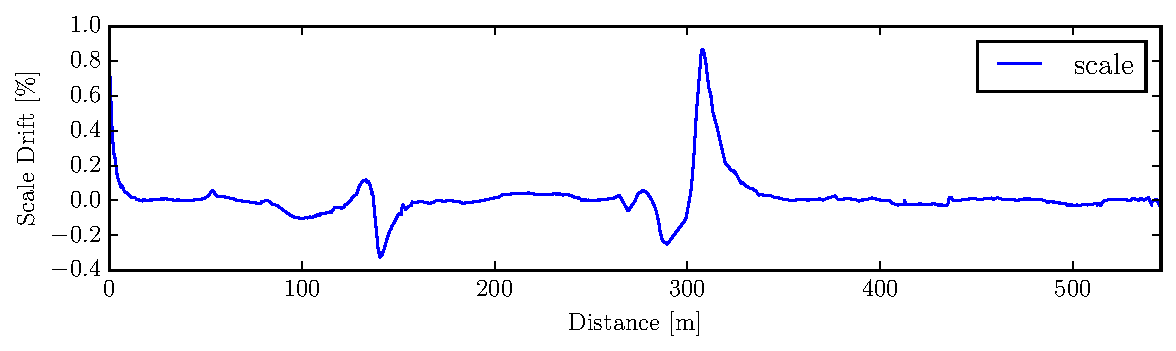
\includegraphics[width=2in]{Chapter4/NTU/server/scale_error_sim3_-1.pdf}
			%\caption{fig2}
		\end{minipage}
	}
\fi
	\caption{Quantitative evaluation results of fused map of NTU Datasets.}
	\label{fig:ntuquanresult}
\end{figure}

\begin{table*}
	\centering
	\caption{Quantitative results of mapping evaluation on Bag.0 NTU Datasets.}
	\begin{threeparttable}
		\begin{tabular}{|c|c|c|c|c|}
			\hline
			Distance(m)\tnote{1} & Rel. Trans.(m)\tnote{2}  & Rel. Trans.($\%$)\tnote{3} & Rel. Yaw(deg)\tnote{4} \\
			\hline
			29& 28.75 & 99.13 & 45.55 \\
			\hline
			58&38.97& 67.19 & 34.89 \\
			\hline
			88&51.96& 59.05 & 43.74  \\
			\hline
			117&37.88&32.38 & 36.31  \\
			\hline
			147&9.29& 6.32 & 10.71 \\
			\hline
		\end{tabular}
		\begin{tablenotes}
			\footnotesize
			\item[1] Distance in meter traveled before each time of statistics. 
			\item[2] Mean relative translation error in meter.
			\item[3] Mean relative translation error in percent.
			\item[4] Mean relative yaw error in degree.
		\end{tablenotes}
	
	\ifoutputscaleerror
			\begin{tabular}{|c|c|c|c|c|}
		\hline
		Distance(m)\tnote{1} & Rel. Trans.(m)\tnote{2}  & Rel. Trans.($\%$)\tnote{3} & Rel. Yaw(deg)\tnote{4} & Scale Err.($\%$)\tnote{5}  \\
		\hline
		29& 28.75 & 99.13 & 45.55& - \\
		\hline
		58&38.97& 67.19 & 34.89 & - \\
		\hline
		88&51.96& 59.05 & 43.74 & - \\
		\hline
		117&37.88&32.38 & 36.31 & - \\
		\hline
		147&9.29& 6.32 & 10.71 & 0.44\\
		\hline
	\end{tabular}
	\begin{tablenotes}
		\footnotesize
		\item[1] Distance in meter traveled before each time of statistics. 
		\item[2] Mean relative translation error in meter.
		\item[3] Mean relative translation error in percent.
		\item[4] Mean relative yaw error in degree.
		\item[5] Median scale error in percent.
	\end{tablenotes}
	\fi

	\end{threeparttable}
	\label{tbl:ntubag0quanresult}
\end{table*}

\begin{table*}
	\centering
	\caption{Quantitative results of mapping evaluation on Bag.1 NTU Datasets.}
	\begin{threeparttable}
		
		\begin{tabular}{|c|c|c|c|c|}
			\hline
			Distance(m)\tnote{1} & Rel. Trans.(m)\tnote{2}  & Rel. Trans.($\%$)\tnote{3} & Rel. Yaw(deg)\tnote{4}   \\
			\hline
			25& 24.79 & 99.17 & 71.03 \\
			\hline
			51&37.20& 72.94 & 88.44  \\
			\hline
			76&29.90& 39.34 & 49.64  \\
			\hline
			102&34.40&33.73& 67.14  \\
			\hline
			127&38.99& 30.70 & 91.89 \\
			\hline
		\end{tabular}
		\begin{tablenotes}
			\footnotesize
			\item[1] Distance in meter traveled before each time of statistics. 
			\item[2] Mean relative translation error in meter.
			\item[3] Mean relative translation error in percent.
			\item[4] Mean relative yaw error in degree.
		\end{tablenotes}
	
	\ifoutputscaleerror
	\begin{tabular}{|c|c|c|c|c|}
		\hline
		Distance(m)\tnote{1} & Rel. Trans.(m)\tnote{2}  & Rel. Trans.($\%$)\tnote{3} & Rel. Yaw(deg)\tnote{4} & Scale Err.($\%$)\tnote{5}  \\
		\hline
		25& 24.79 & 99.17 & 71.03 & - \\
		\hline
		51&37.20& 72.94 & 88.44 & - \\
		\hline
		76&29.90& 39.34 & 49.64 & - \\
		\hline
		102&34.40&33.73& 67.14 & - \\
		\hline
		127&38.99& 30.70 & 91.89 & -1.31\\
		\hline
	\end{tabular}
	\begin{tablenotes}
		\footnotesize
		\item[1] Distance in meter traveled before each time of statistics. 
		\item[2] Mean relative translation error in meter.
		\item[3] Mean relative translation error in percent.
		\item[4] Mean relative yaw error in degree.
		\item[5] Median scale error in percent.
	\end{tablenotes}
\fi
	\end{threeparttable}
	\label{tbl:ntubag1quanresult}
\end{table*}

\begin{table*}
	\centering
	\caption{Quantitative results of map fusion evaluation on  NTU Datasets.}
	\begin{threeparttable}
		\begin{tabular}{|c|c|c|c|c|}
			\hline
			Distance(m)\tnote{1} & Rel. Trans.(m)\tnote{2}  & Rel. Trans.($\%$)\tnote{3} & Rel. Yaw(deg)\tnote{4}  \\
			\hline
			54& 39.38 & 72.93 & 44.39 \\
			\hline
			109&44.88& 41.18 & 57.01  \\
			\hline
			163&26.09& 16.00 & 32.12  \\
			\hline
			218&54.99& 25.23 & 46.11  \\
			\hline
			272&64.66& 23.77 & 54.65 \\
			\hline
		\end{tabular}
		\begin{tablenotes}
			\footnotesize
			\item[1] Distance in meter traveled before each time of statistics. 
			\item[2] Mean relative translation error in meter.
			\item[3] Mean relative translation error in percent.
			\item[4] Mean relative yaw error in degree.
		\end{tablenotes}
	
	\ifoutputscaleerror
			\begin{tabular}{|c|c|c|c|c|}
		\hline
		Distance(m)\tnote{1} & Rel. Trans.(m)\tnote{2}  & Rel. Trans.($\%$)\tnote{3} & Rel. Yaw(deg)\tnote{4} & Scale Err.($\%$)\tnote{5}  \\
		\hline
		54& 39.38 & 72.93 & 44.39& - \\
		\hline
		109&44.88& 41.18 & 57.01 & - \\
		\hline
		163&26.09& 16.00 & 32.12 & - \\
		\hline
		218&54.99& 25.23 & 46.11 & - \\
		\hline
		272&64.66& 23.77 & 54.65 & 0.10\\
		\hline
	\end{tabular}
	\begin{tablenotes}
		\footnotesize
		\item[1] Distance in meter traveled before each time of statistics. 
		\item[2] Mean relative translation error in meter.
		\item[3] Mean relative translation error in percent.
		\item[4] Mean relative yaw error in degree.
		\item[5] Median scale error in percent.
	\end{tablenotes}
\fi
	\end{threeparttable}
	\label{tbl:ntuquanresult}
\end{table*}
